\documentclass[a4paper]{article}

%% Language and font encodings
\usepackage[english]{babel}
\usepackage[utf8x]{inputenc}
\usepackage[T1]{fontenc}
\usepackage{lipsum}
% \renewcommand\Authfont{\fontsize{12}{14.4}\selectfont}

%% Sets page size and margins
\usepackage[a4paper,top=1.5cm,bottom=1.75cm,left=1.5cm,right=1.5cm,marginparwidth=2cm]{geometry}

%% Useful packages
\usepackage{amsmath}
\usepackage{graphicx}
\usepackage[colorinlistoftodos]{todonotes}
\usepackage[colorlinks=true, allcolors=blue]{hyperref}

\title{\textbf{ARM11 Final Report}}
\author{
  Ashvin Arsakularatne\\
  \texttt{aa9220@ic.ac.uk}
  \and
  Kavya Chopra\\
  \texttt{kc2320@ic.ac.uk}
  \and
  Siddhant Singh\\
  \texttt{ss5120@ic.ac.uk}
  \and
  Ye Lun Yang\\
  \texttt{yly19@ic.ac.uk}
}

\begin{document}
\maketitle

\section{Assembler}
\subsection{The structure:}
\subsubsection{First Pass: }
During the first pass, the assembler initialises the linked list and the symbol table using the \verb|init_linked_list()| and \verb|init_symbol_table()| respectively in \verb|assemble.c|. The linked list is initialised by setting the head to \verb|NULL| and allocating memory based on the size of the linked list. The symbol table is initialised by allocating contiguous memory, setting the capacity to \verb|64| and the key-value pairs to \verb|NULL|. Once the symbol table is initialised, we populate the table with function mappings for all pre-defined instructions mentioned in spec. The instruction function mappings are a combination of a \verb|union| code and a parse functional pointer pointing to the appropriate parse function. 

Once the structures have been initialised, lines from the \verb|.s| file are read (all being of length \verb|511| as specified by the spec), trailing whitespace from each line is removed and any erroneous line is ignored. Then, the line is tokenised using the \verb|tokenizer()| function in \verb|tokenizer.c|. The tokenized instruction is then appended to the linked list. Thus, the length of the link list will be 1 more than the number of lines in the \verb|.s| file (as the head is \verb|NULL|). 

Before adding to the linked list, a node is initialised using a simple memory allocation (\verb|malloc|) and each allocation is double checked to make sure the memory allocation is a success, if it isn't, a \verb|perror()| is thrown. This linked list is passed to the parser which is part of the second pass.

\subsubsection{Second Pass: }
First, we open the file for writing in binary (\verb|wb| mode in C). In the second pass, we apply the parsing functions to each node in the linked list as shown in Figure \ref{fig:assembler}. We first check which type of instruction it is and then pass the contents of the node into the respective functions (\verb|parse_dataproc| for data processing instructions, \verb|parse_mult| for multiplication instructions, \verb|parse_sdt| for single data transfer instructions, \verb|parse_branch| for branch instructions and \verb|parse_lsl| for the special \verb|lsl| instruction). The intricacies of these functions will be covered in sub-section \ref{Assembler implementation}. 

Once the parse operations have been performed, the parsed instruction will be sent to the respective binary encoder. The encoder performs simple bitwise operations on a \verb|uint32_t| integer which is then returned by the parse function where it was called. Once encoded, \verb|write_file()| is called and the encoded binary is written to the file opened before the linked list iteration had begun. This process repeats for every node in the linked list (apart from the head) and once the iteration ends, all allocated memory is freed (symbol table, linked list, linked list nodes etc.) and the file is closed.

\begin{figure}[htp]
    \centering
    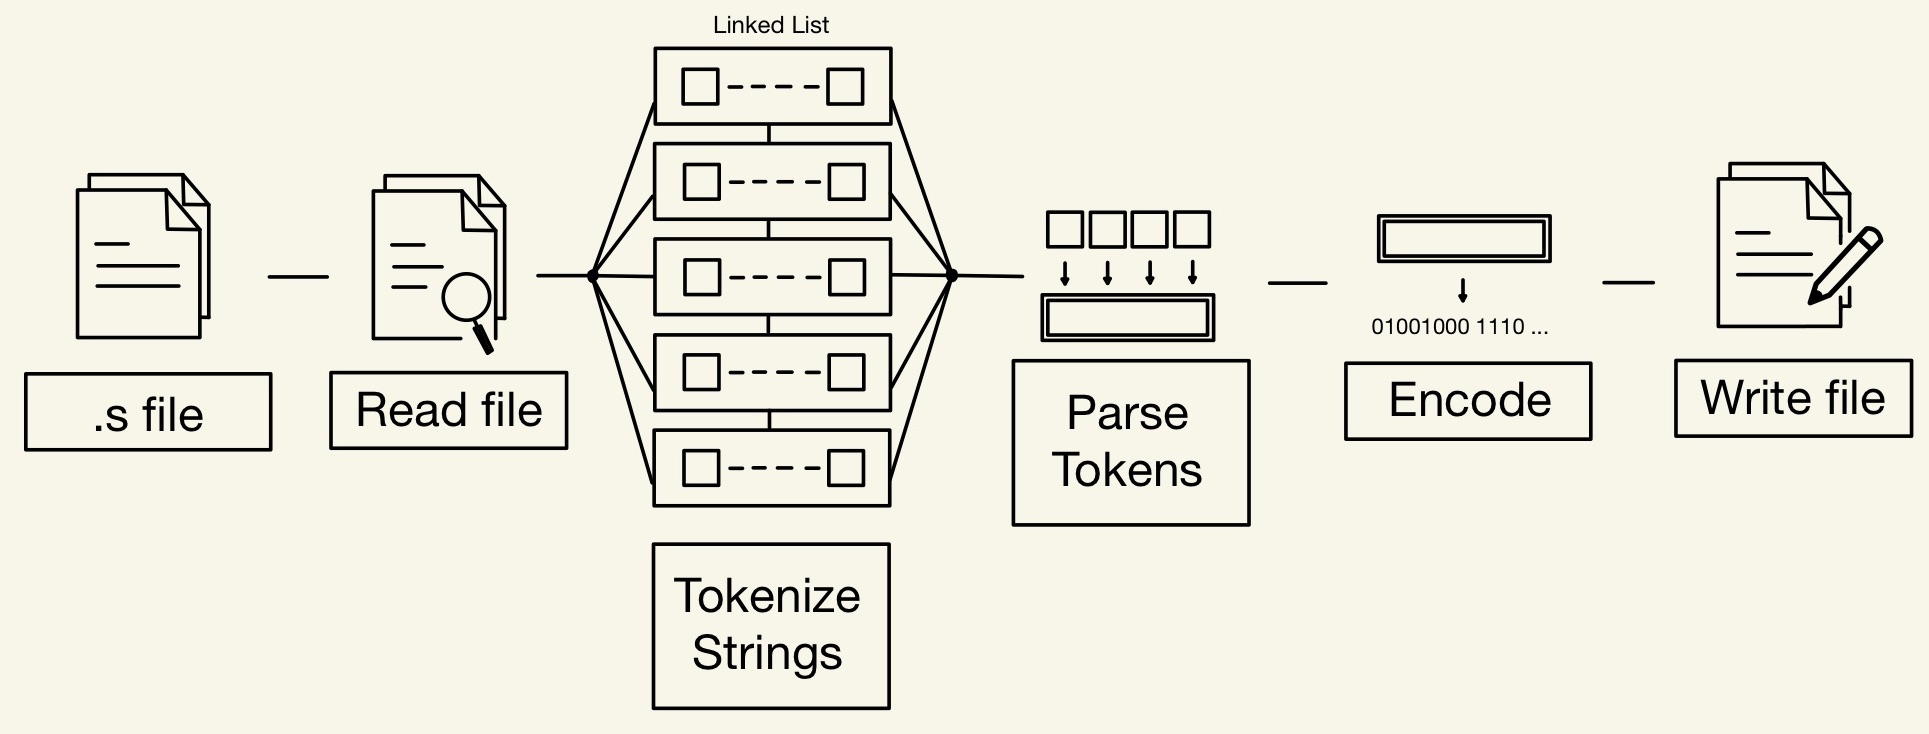
\includegraphics[width=15cm]{assembler_flowchart.jpg}
    \caption{Our 2-pass assembly process}
    \label{fig:assembler}
\end{figure}

\subsection{The implementation:}\label{Assembler implementation}
% Why we chose a 2-pass approach
% Talk about the functional pointers 
% Decision choice about using parser and encoder in one function
% How the tokenizer works
% Some detail on parse_operand2()

Reading from the source file is required to obtain our instructions in string form. We decided to take the two-pass approach when tackling the assembler.

A notable issue we faced was that we did not know how many lines there were in each source file, so we could not create an array of strings to store these instructions. To tackle this, we used a linked list to store the instructions instead. Since we took such an approach, we could then read through the source file once, converting each instruction in a tokenized form and inserting them into the linked list. Labels are inserted into our symbol table, and are not inserted into the linked list.

\section{Extension: A Concurrent Application of Blockchain Mining in C}
\subsection{Real world usage:}
\lipsum[1-1]
\subsection{The implementation:}
\lipsum[1-1]
\subsection{Testing:}
\lipsum[1-1]
\subsubsection{Effectiveness of testing:}
\lipsum[1-1]

\section{Group Reflection}
\subsection{Effectiveness of communication and division of work:}
\lipsum[1-1]
\subsection{Future improvements:}
\lipsum[1-1]

\section{Individual Reflections}
\subsection{Ashvin:}
\lipsum[1-1]
\subsection{Kavya:}
\lipsum[1-1]
\subsection{Siddhant:}
\lipsum[1-1]
\subsection{Ye Lun:}
\lipsum[1-1]

\end{document}